%% LyX 2.2.2 created this file.  For more info, see http://www.lyx.org/.
%% Do not edit unless you really know what you are doing.
\documentclass[english]{article}
\usepackage[T1]{fontenc}
\usepackage[latin9]{inputenc}
\usepackage{geometry}
\geometry{verbose,tmargin=3cm,bmargin=5cm,lmargin=3cm,rmargin=3cm}
\usepackage{babel}
\usepackage{array}
\usepackage{wrapfig}
\usepackage{graphicx}
\usepackage[unicode=true]
 {hyperref}

\makeatletter

%%%%%%%%%%%%%%%%%%%%%%%%%%%%%% LyX specific LaTeX commands.
%% Because html converters don't know tabularnewline
\providecommand{\tabularnewline}{\\}
%% A simple dot to overcome graphicx limitations
\newcommand{\lyxdot}{.}


\makeatother

\begin{document}

\title{Cicuta}

\maketitle
Sample document content taken from this Wikipedia page: \href{https://en.wikipedia.org/wiki/Cicuta}{https://en.wikipedia.org/wiki/Cicuta}.
All images are in the public domain.

\medskip{}

\begin{wrapfigure}{o}{0.5\columnwidth}%
\begin{centering}
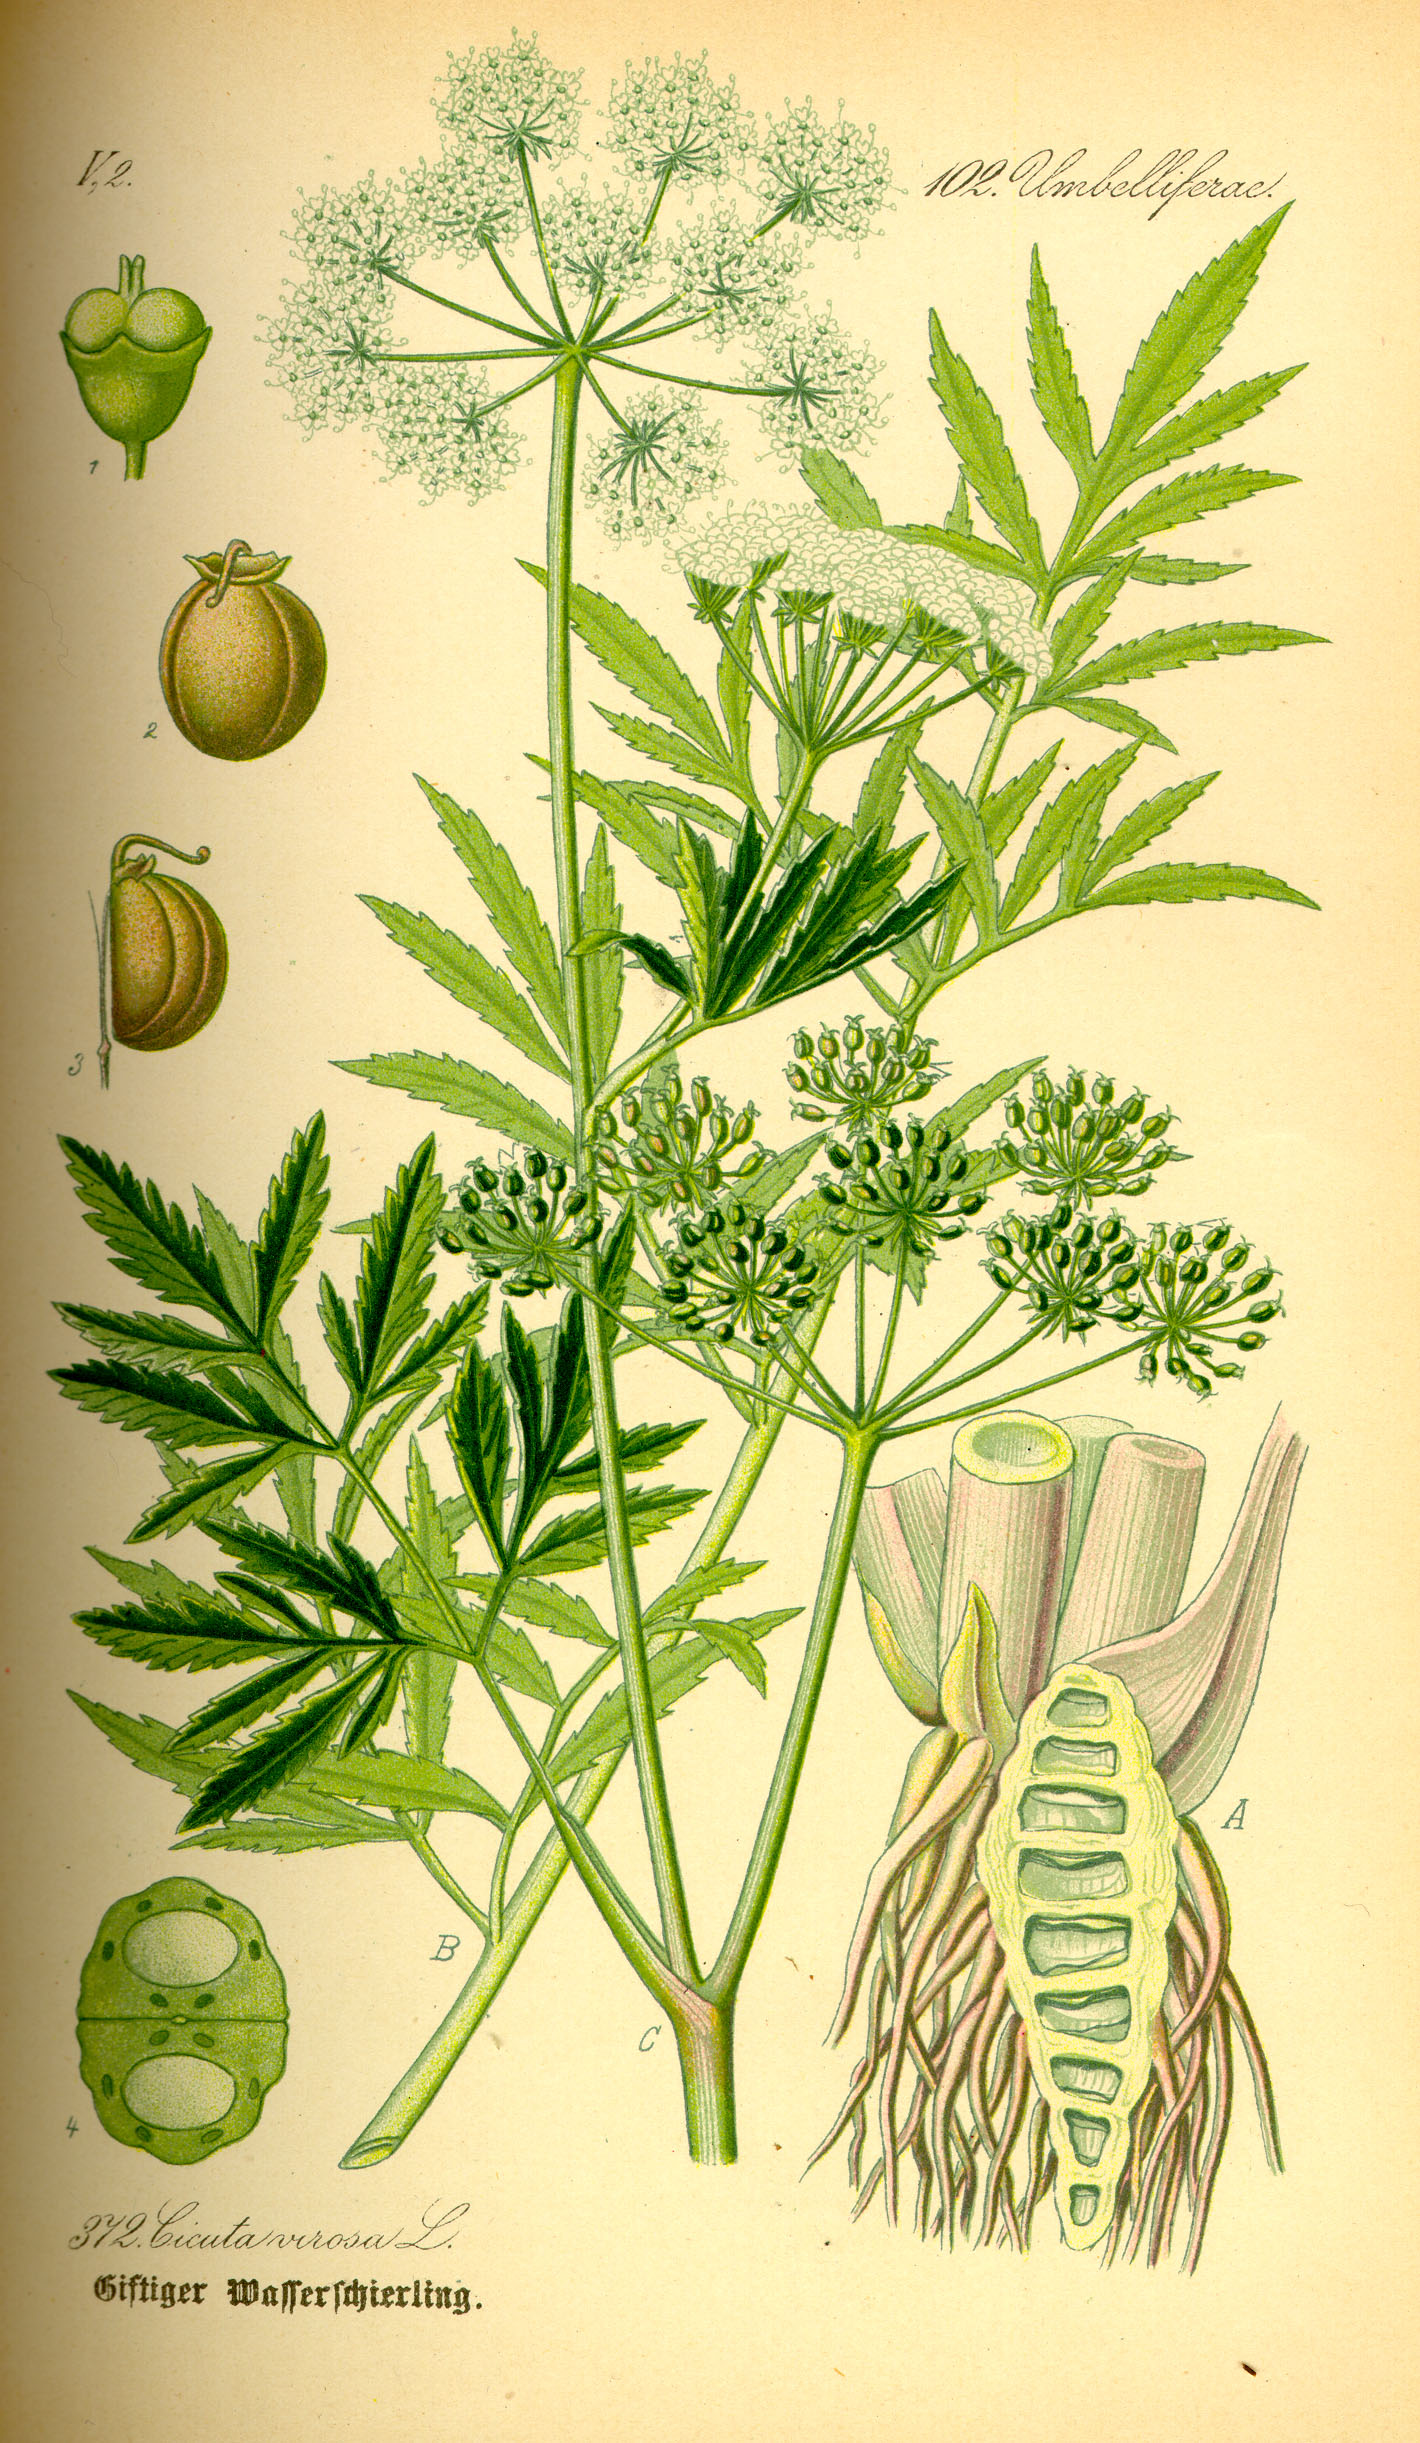
\includegraphics[width=4cm]{IllustrationCicutaVirosa0}
\par\end{centering}
\caption{Cicuta Virosa. }
\end{wrapfigure}%
Cicuta, commonly known as water hemlock, is a small genus of four
species of highly poisonous plants in the family Apiaceae. They are
perennial herbaceous plants which grow up to 2.5 meters (8.2 ft) tall,
having distinctive small green or white flowers arranged in an umbrella
shape (umbel). Plants in this genus may also be referred to as cowbane
or poison parsnip. Cicuta is native to temperate regions of the Northern
Hemisphere, mainly North America and Europe, typically growing in
wet meadows, along streambanks and other wet and marshy areas. These
plants bear a close resemblance to other members in the family Apiaceae
and may be confused with a number of other edible and poisonous plants.
The common name hemlock may also be confused with poison hemlock (Conium
maculatum).

Water hemlock is considered one of North America's most toxic plants,
being highly poisonous to humans.{[}1{]} Three members of the genus
contain a toxin named cicutoxin which causes central nervous system
stimulatory effects including seizures following ingestion. Medical
treatment of poisoning may include the use of activated charcoal to
decrease gastrointestinal absorption of the toxic principle along
with supportive care including anticonvulsant drugs such as a benzodiazepine.
High doses of anticonvulsant medicine are often required to halt seizure
activity and further medical care including intubation and mechanical
ventilation may be required.

\section{Description}

\begin{figure}
\begin{centering}
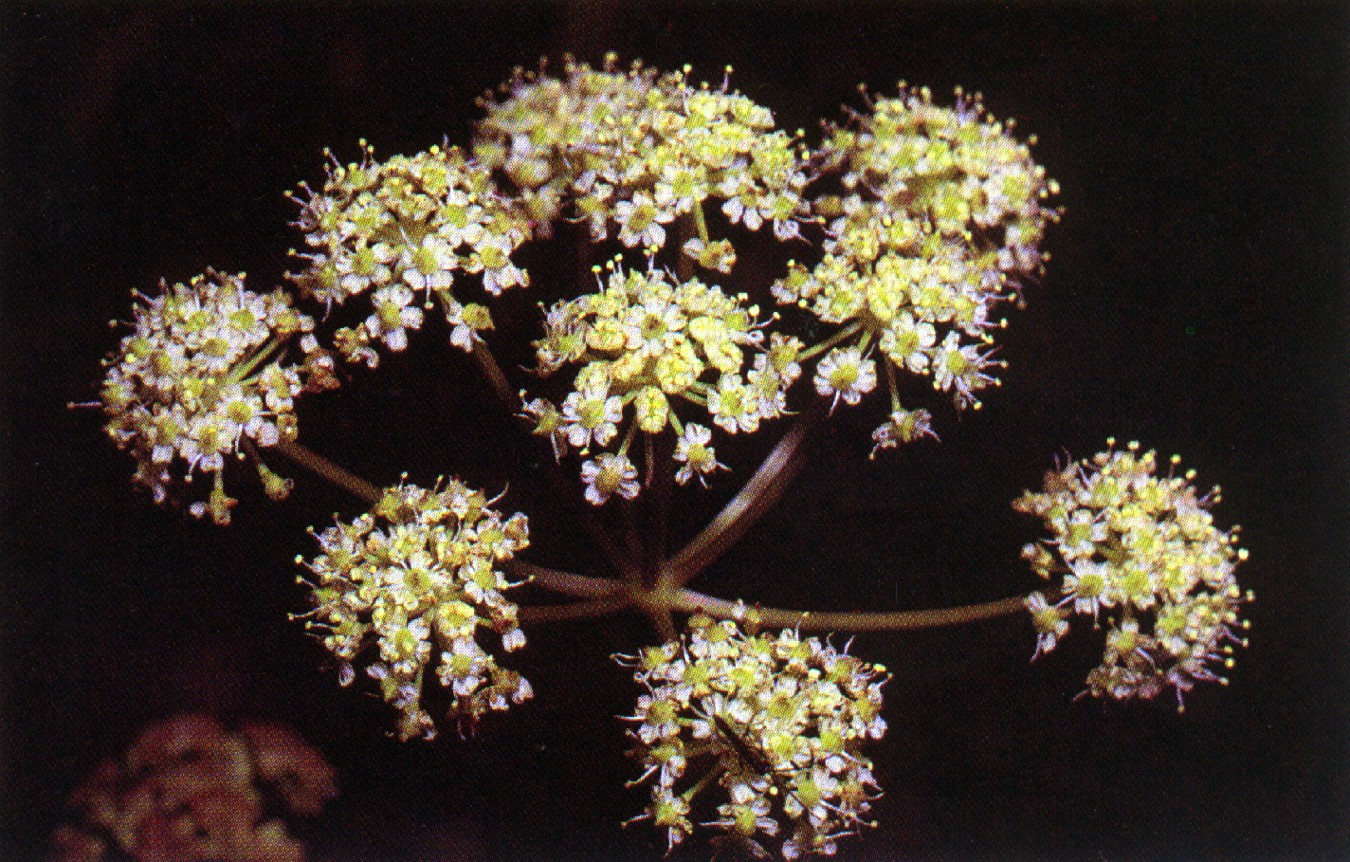
\includegraphics[width=6cm]{CicutaDouglasii}
\par\end{centering}
\caption{Cicuta douglasii, showing the umbrella shaped umbel.}

\end{figure}

Cicuta spp. are perennial plants that are all similar in morphology,
growing up to a maximum of 2.5 meters (8.2 ft) in height. The stem
of the plant is branching, erect, smooth and hollow (except for partitions
at the junction of the leaves and stem), sometimes being purple-striped,
or mottled (typically only C. maculata has the purple stripes or spots).
Attached to the base of the stem is a tuberous root with thickened
rootstocks. The rootstocks are multichambered and contain a yellowish
oily liquid which turns reddish brown on exposure to air and emits
a characteristic smell of raw parsnip. The alternate leaves are 2
or 3 pinnately compound and may reach 30 centimeters (12 in) to 90
centimeters (35 in) in length. The leaflets are lanceolate, serrate,
5 centimeters (2.0 in) to 10 centimeters (3.9 in) in length, and sharply
toothed. The plant flowers in spring or early summer; the flowers
are small with green or white petals clustered in an umbrella shape
(umbel) characteristic to this family; the umbel measures 5 centimeters
(2.0 in) to 10 centimeters (3.9 in) across. The plants produce a cylindrical
fruit which is 4 millimeters (0.16 in) to 6 millimeters (0.24 in)
in length.{[}1{]}{[}2{]}{[}3{]} The plant is spread primarily by seeds
which are produced in large numbers and are small in size.{[}2{]}

\section{Taxonomy}

The Cicuta genus is one of many genera in the Apiaceae family which
is in the order Apiales. The Apiaceae family is also known as Umbelliferae
and both of these family names are permitted to be used by the International
Code of Botanical Nomenclature.{[}1{]} In Europe, Cicuta was not distinguished
from the similar genus Conium before the year 1500. The first mention
of the genus in the United States was in the eighteenth century.{[}2{]}
Carl Linnaeus formally described three species in 1753.{[}4{]} The
type species is Cicuta virosa.{[}5{]} The genus is now recognized
to comprise four species:{[}6{]}
\begin{center}
\begin{tabular}{|>{\raggedright}p{4cm}|>{\raggedright}p{5cm}|}
\hline 
Species Name & Common Name\tabularnewline
\hline 
\hline 
Cicuta bulbifera L. & bulblet-bearing water hemlock, bulbous water hemlock \tabularnewline
\hline 
Cicuta douglasii (DC.) Coult. \& Rose  & Douglas water hemlock, western water hemlock \tabularnewline
\hline 
Cicuta maculata L.  & spotted cowbane, spotted parsley, spotted water hemlock \tabularnewline
\hline 
Cicuta virosa L. & cowbane, Mackenzie\textquoteright s water hemlock, northern water
hemlock \tabularnewline
\hline 
\end{tabular}
\par\end{center}

Other species names such as Cicuta bolanderi, Cicuta californica,
and Cicuta curtissii are older names now recognized to be varieties
of the widespread, morphologically variable Cicuta maculata.{[}3{]}
Cicuta maculata is now recognized to have four varieties: var. maculata,
var. augustifolia, var. victorinii, and var. bolanderi.{[}6{]} Phylogenetic
analysis using the sequences of nuclear ribosomal DNA internal transcribed
spacer (ITS) loci was not conclusive but seems to show that C. bulbifera
and C. virosa are monophyletic, while C. douglasii may not be. It
was also suggested a specimen from California may warrant recognition
as a distinct species.{[}7{]} Other common names for the genus in
general include poison parsnip, beaver poison, wild carrot, wild parsnip,
and false parsley.{[}8{]}

\section{Similar Species}

Members of the family Apiaceae bear close resemblance to each other,
and have many characteristics in common. Cicuta spp. are often mistaken
for edible plants such as kvanne (Angelica archangelica), wild celery
(Apium graveolens), pignut (Conopodium majus), wild carrot (Daucus
carota), wild parsnip (Pastinaca sativa), and water parsnip (Berula
spp.).{[}1{]} One of the more common misidentifications is between
water hemlock and water parsnip; both have clusters of small white
flowers shaped like umbrellas, and both have the same habitat near
the shore line of lakes and rivers. Differences between water parsnip
and water hemlock include the water parsnip having leaves only once
compound while the water hemlock has leaves which are two or three
times compound. Water hemlock also has a large swelling at the stem
base which water parsnip lacks. Additionally, water hemlock has bracts
at the base of each small flower cluster, not at the base of the main
flower head,{[}9{]} while water parsnip has both bracts at the base
of flowers and also at the main flower head.{[}10{]}

\begin{figure}
\begin{centering}
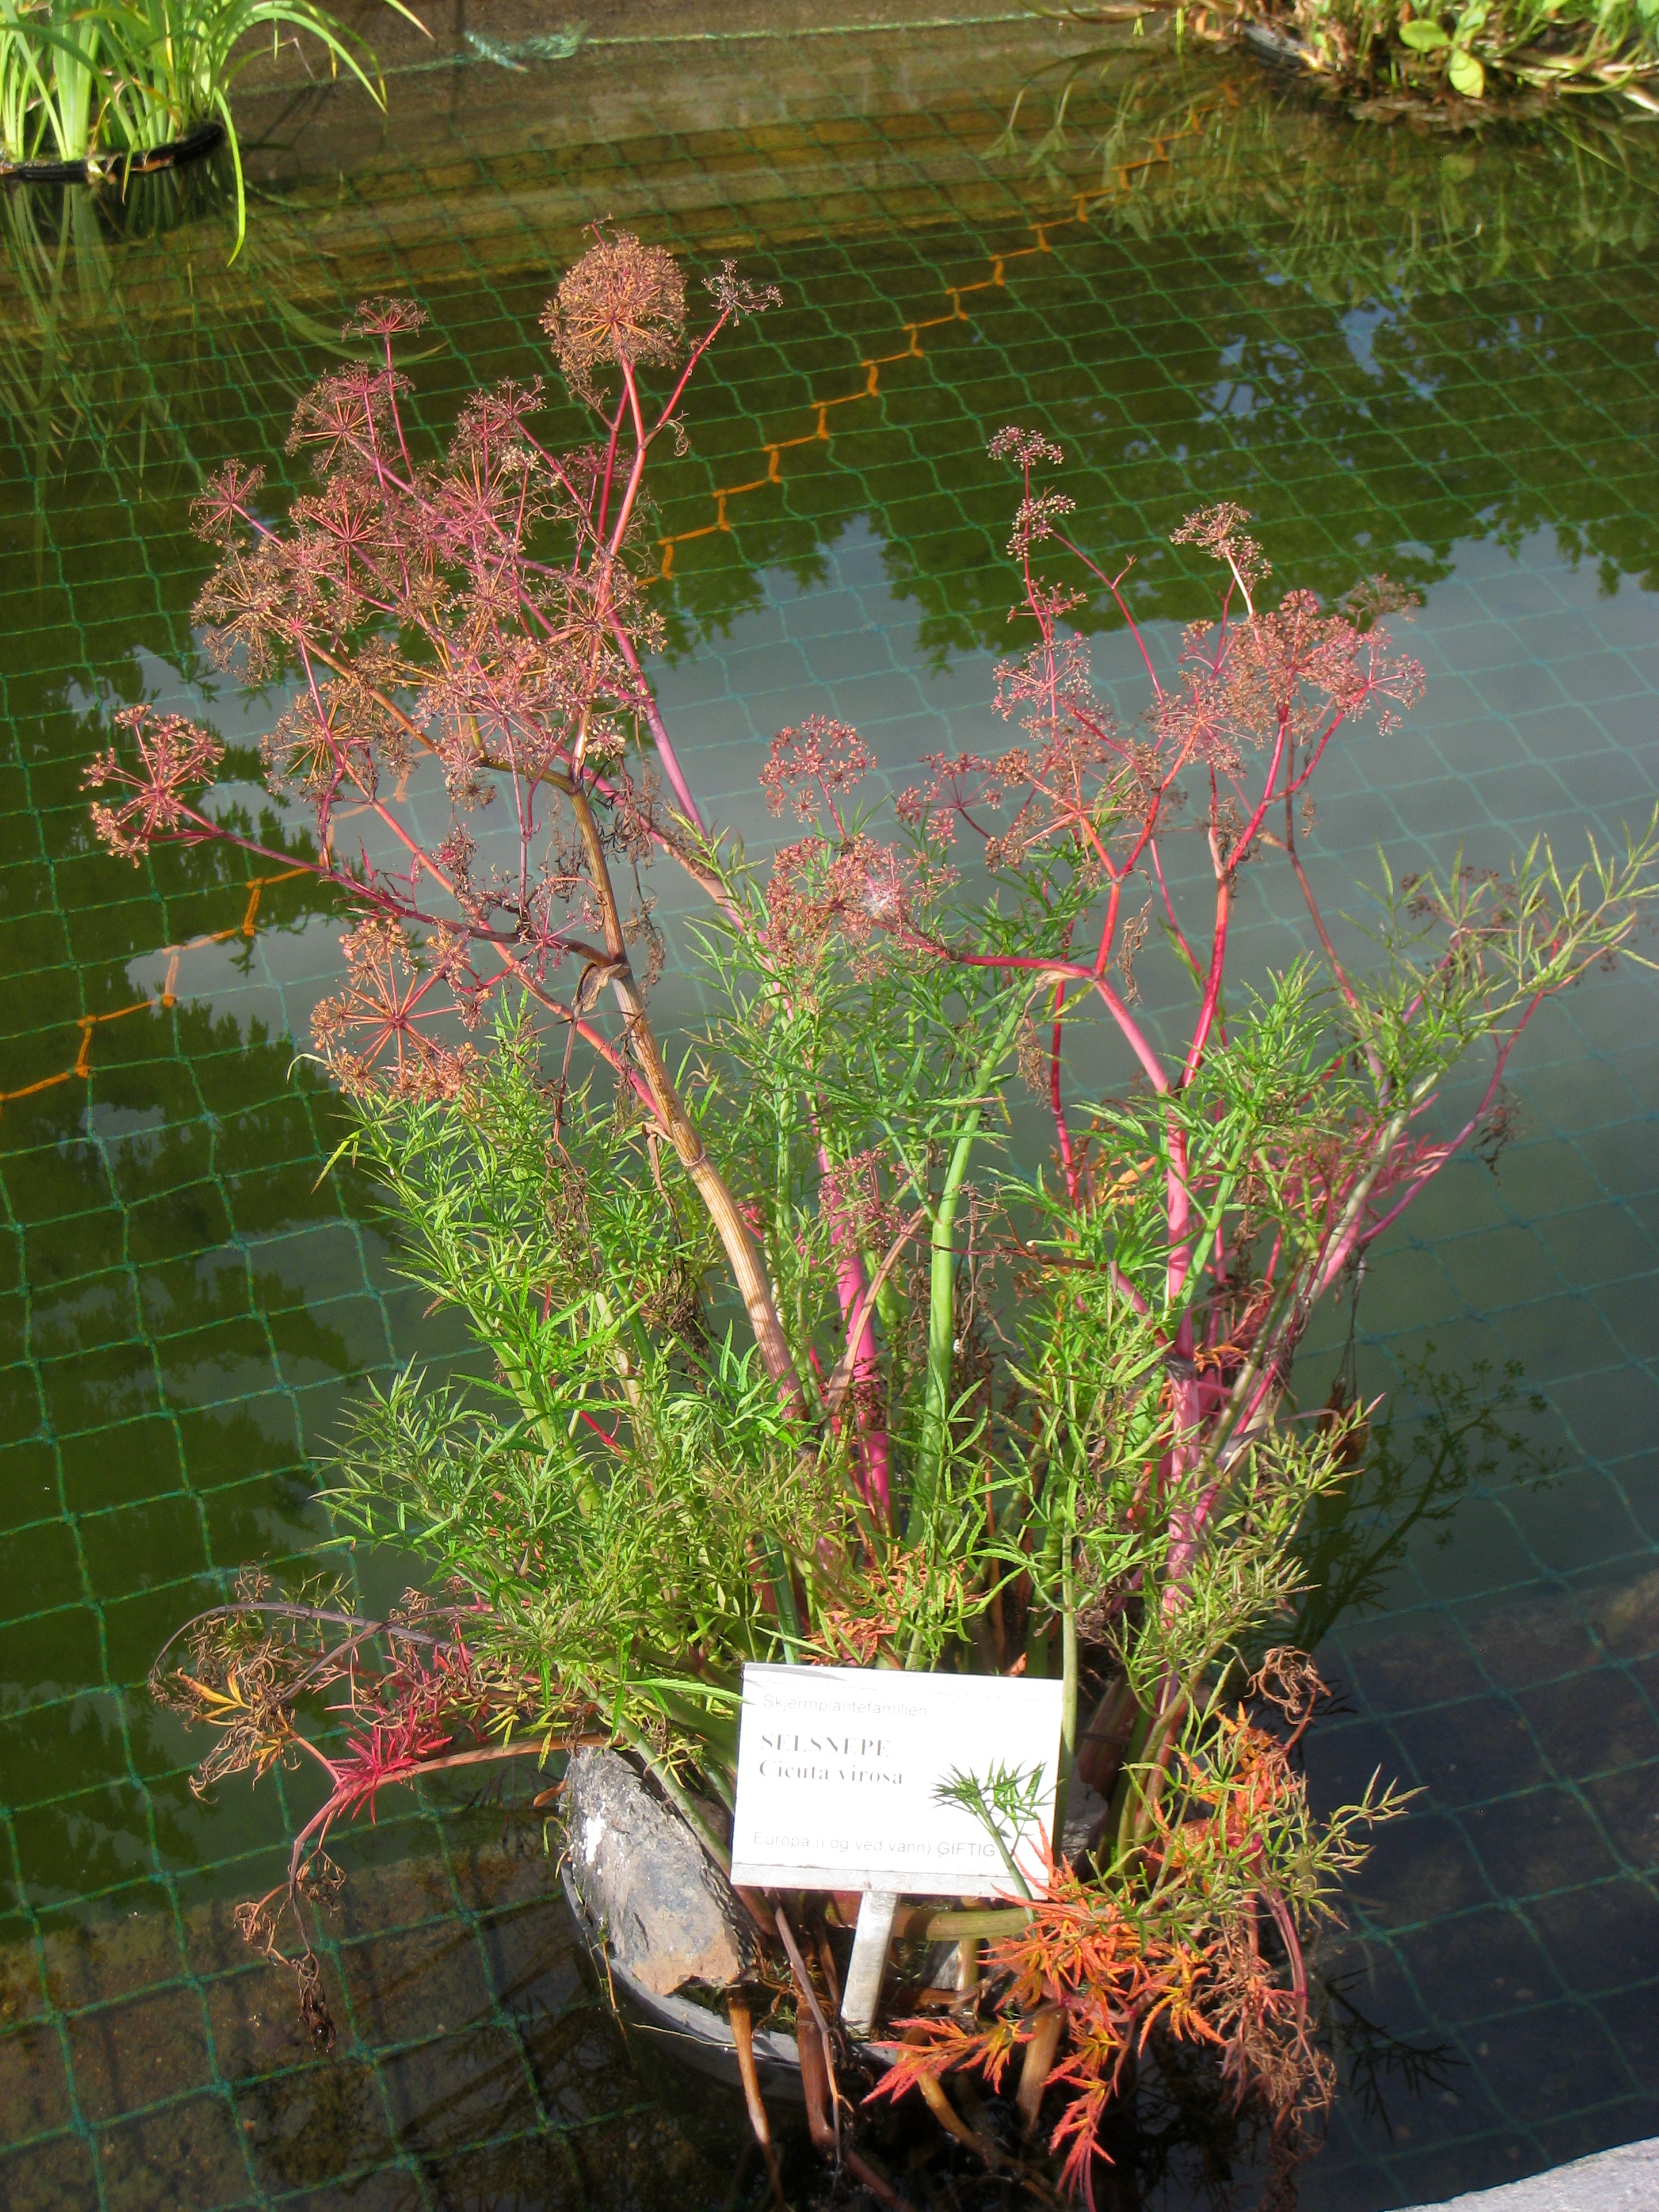
\includegraphics[width=5cm]{CicutaVirosa--OsloBotanicalGarden--IMG8917}
\par\end{centering}
\caption{Cicuta virosa}

\end{figure}

Additionally, there can be confusion between the various water hemlock
species and poison hemlock (Conium maculatum){[}11{]} as the common
name hemlock is applied to both Cicuta and Conium maculatum.{[}12{]}
Both are poisonous and can be differentiated by differences in their
root structure. Water hemlock has a branched root systems with tubules,
while poison hemlock has a single tap root.{[}1{]} Another reliable
method to identify water hemlock is to examine the leaf veins. Water
Hemlock is unique in the Apiaceae family in that it has leaf veins
which terminate in the notches between the leaf tips, rather than
extend to the tip of the leaf, as is found in the leaf structure of
other members of this family.{[}2{]}

\section{Distribution and habitat}

Cicuta spp. are found growing across North America and Europe. Typically,
they grow in wet habitats usually alongside ponds and streams, in
marshes or swamps, or areas that are swampy at least part of the year.
Plants can also be found growing in water.{[}2{]}{[}3{]} Of the four
species, Cicuta maculata has the most widespread distribution occurring
across the majority of North America. Cicuta bulbifera also has a
relatively large distribution, found throughout Northern North America.
Cicuta douglasii is found in the northwest corner of North America,
while Cicuta virosa is only found in central Europe and in the far
north of North America.{[}1{]}{[}3{]}

\section{Toxicity}

All members of Cicuta except C. bulbifera contain high levels of the
poisonous principle cicutoxin, an unsaturated aliphatic alcohol that
is structurally closely related to the toxin oenanthotoxin found in
the plant hemlock water dropwort. Cicutoxin is present at all stages
of growth and in all parts of the plant, but is most concentrated
in the roots which appear to be the most toxic in the early spring.{[}1{]}
Its primary toxic effect is to act as a stimulant in the central nervous
system. It is a non-competitive gamma-aminobutyric acid (GABA) receptor
antagonist. Cicutoxin acts on the GABAA receptor causing a block of
the chloride channel which results in neuronal depolarization. In
the presence of cicutoxin this depolarization continues unabated causing
cell overactivity. The hyperactivity in brain cells results in seizures.{[}1{]}{[}13{]}
Cicutoxin is highly poisonous and water hemlock is considered one
of North America's most toxic plants.{[}1{]}{[}14{]} Ingestion of
Cicuta can be fatal in humans and there are reports in the medical
literature of severe poisoning and death as early as 1670.{[}1{]}
A number of people have also died following ingestion of the plant
in the 20th and 21st century.{[}8{]}{[}15{]}{[}16{]}{[}17{]}{[}18{]}{[}19{]}

The LD50 in mice administered cicutoxin by intraperitoneal injection
is 48.3 mg per kg body weight (mg/kg); this compares with 5.9 mg/kg
for mice given potassium cyanide by intraperitoneal injection, while
the LD50 for arsenic via intraperitoneal injection in mice is 46.2
mg/kg.{[}20{]} The exact toxic dose of plant material in humans is
unknown; it is thought ingestion of water hemlock in any quantity
can result in poisoning and very small amounts may lead to death.{[}1{]}
Poisoning has been reported following children blowing whistles made
from the hollow stem of water hemlock plants.{[}21{]} Intoxication
has also been reported following skin contact with the plant; a case
was reported where a family of five people rubbed the plant onto the
skin and were poisoned, with two children dying.{[}22{]} Livestock
have long been the worst affected, leading to the common name \textquotedbl{}cowbane\textquotedbl{}.
Poisoning in livestock is common and typically occurs following ingestion
of roots of the plant. In the spring when the ground is soft, grazing
animals tend to pull the entire plant out of the ground ingesting
both the foiliage and the roots. Roots exposed by ploughing can also
be the source of livestock poisonings.{[}2{]} Ingestion of plant material
may cause death in the animal in as little as 15 minutes.{[}23{]}{[}24{]}{[}25{]}

\begin{figure}
\begin{centering}
\includegraphics[width=5cm]{500px-Cicutoxin\lyxdot svg}
\par\end{centering}
\caption{Cicutoxin is the major poison in Cicuta spp. plants.}

\end{figure}


\subsection{Symptoms}

Upon consumption, both in humans and other species, the symptoms of
poisoning are mainly characterized by generalized seizures.{[}1{]}
The onset of symptoms following ingestion may be as soon as 15 minutes
post ingestion. Initial symptoms reported may include nausea, vomiting,
abdominal pain, tremors, confusion, weakness, dizziness, and drowsiness;{[}14{]}{[}26{]}
although the rapid onset of seizure activity may be the first sign
presented following poisoning. Seizures are usually described as clonic
or tonic\textendash clonic.{[}1{]} Complications of ongoing seizure
activity include increased body temperature, decreases in the pH of
the blood (metabolic acidosis), swelling in the brain, blood coagulation
disorders, muscle breakdown (rhabdomyolysis), and kidney failure.{[}1{]}{[}27{]}{[}28{]}
Additional neurological symptoms may include hallucinations, delirium,
tingling, pricking, or numbness of a person's skin, dilated pupils,
and coma.{[}1{]}{[}14{]} Cardiovascular symptoms include alternating
slow or fast heart rate{[}29{]} and alternating low and high blood
pressure.{[}30{]} Other cardiac effects may include ECG abnormalities
such as widening of the PR interval, supraventricular tachycardia,
and ventricular fibrillation.{[}1{]}{[}15{]}{[}31{]} Symptoms of excess
salivation, wheezing, respiratory distress, and absence of breathing
have also been reported.{[}1{]}{[}26{]}

Deaths usually occur from respiratory failure or ventricular fibrillation
secondary to ongoing seizure activity;{[}1{]} fatalities have occurred
within a few hours of ingestion.{[}3{]} Poisoned people who recover
usually regain consciousness and seizures cease within 24 to 48 hours
of poisoning, although seizures may persist for up to 96 hours.{[}1{]}
There are occasional long-term effects such as retrograde amnesia
of the events leading to intoxication and the intoxication itself.{[}8{]}{[}26{]}{[}30{]}{[}32{]}
Other ongoing mild effects may include restlessness, muscle weakness,
twitching, and anxiety.{[}1{]}{[}33{]} Complete resolution of symptoms
may take a number of days or, in some cases, these ongoing symptoms
may persist for months after poisoning.{[}1{]}

\subsection{Diagnosis and treatment}

Water hemlock poisoning is usually diagnosed following a history of
plant ingestion and symptoms of abrupt onset of seizures.{[}16{]}{[}34{]}
Laboratory tests to determine the presence of cicutoxin in the blood
such as spectrofluorimetry, high pressure liquid chromatography, thin
layer chromatography, and mass spectrometry have been used to detect
cicutoxin but these tests are not performed routinely in hospital
laboratories.{[}1{]}{[}35{]} If a sample of the plant ingested has
been retained, diagnosis can be confirmed by having the plant identified
by a botanist.{[}1{]}

Initial treatment of poisoning may include gastrointestinal decontamination
with activated charcoal.{[}35{]} Decontamination is typically only
performed if a potentially toxic amount of plant matter has been ingested
up to one hour previously and the patient has a normal intact airway
or has been intubated.{[}1{]} There is no specific antidote for water
hemlock poisoning and treatment mainly consists of supportive care.
Treatment may include control of seizures with the administration
of a benzodiazepines such as lorazepam or diazepam, or if seizures
are refractory to this treatment, a barbiturate such as phenobarbital
is administered.{[}1{]} The anticonvulsant phenytoin is not recommended
as it has not been shown to be effective for seizure control following
water hemlock poisoning.{[}34{]} Treatment with high doses of benzodiazepines
or barbiturates may cause respiratory depression and respiratory support
including intubation and mechanical ventilation is required in these
patients.{[}1{]} Continuous electroencephalography monitoring is recommended
in symptomatic patients.{[}1{]}

Further treatment for complications of metabolic acidosis, rhabdomyolysis,
hyperthermia, or low blood pressure may be required. Metabolic acidosis
is treated by administering sodium bicarbonate.{[}36{]} Low blood
pressure is usually treated with intravenous fluid replacement, but
the administration of dopamine or norepinephrine may be required to
restore blood pressure.{[}1{]}{[}35{]} The management of rhabdomyolysis
includes ensuring adequate hydration and urinary alkalinization; a
complication of rhabdomyolysis is acute renal failure which may require
management with hemodialysis.{[}1{]} However, hemodialysis, hemoperfusion
or other extracorporeal techniques do not remove cicutoxin from the
blood and are therefore not useful in enhancing elimination.{[}1{]}{[}35{]}
\end{document}
